


À chaque fois que le module reçoit une annotation, celui-ci effectue une mise à jour des probabilité
\[ P(Annotation|Forme) = \frac{P(Annotation|Gain) \times P(Gain)}{P(Annotation)} \]

Par exemple, imaginons que nous souhaitons entraîner notre IA à identifier des formes géométrique basique : rond, carré, croix et triangle. Admettons que notre IA est capable de reconnaître dans son environnement les formes correspondantes mais qu'elle ne sait pas les associer au concept correspondant. Nous pouvons représenter cette état par le tableau représenté en figure \ref{img_annotations}.

\begin{figure}[H] 
  \begin{center}
    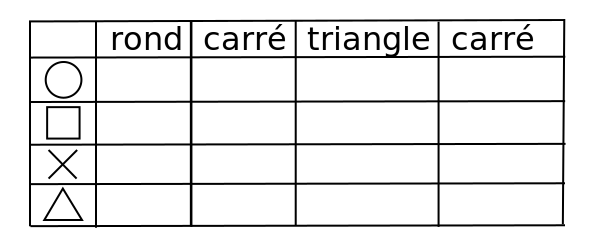
\includegraphics[width=0.5\textwidth]{files/raisonneur/annotations} 
  \end{center}
\caption{Association forme-concept} 
\label{img_annotations}
\end{figure}

\begin{figure}[H] 
\includegraphics[width=\textwidth]{files/raisonneur/annotations_1} 
\caption{Association forme-concept 1} 
\label{img_annotations_1}
\end{figure}

\begin{figure}[H] 
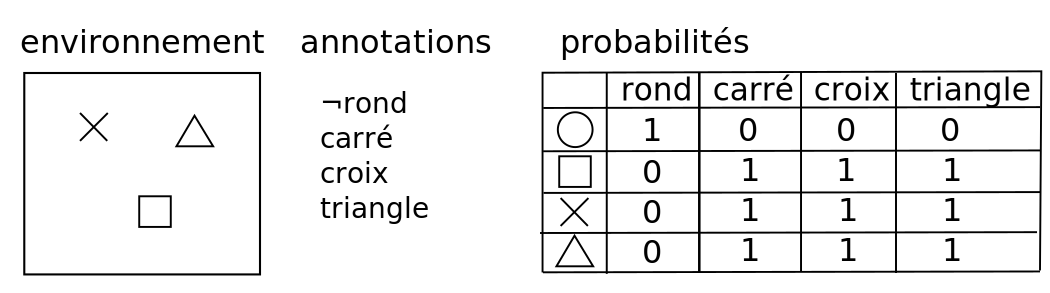
\includegraphics[width=\textwidth]{files/raisonneur/annotations_2} 
\caption{Association forme-concept 2} 
\label{img_annotations_2}
\end{figure}

\begin{figure}[H] 
\includegraphics[width=\textwidth]{files/raisonneur/annotations_3} 
\caption{Association forme-concept 3} 
\label{img_annotations_3}
\end{figure}

\begin{figure}[H] 
\includegraphics[width=\textwidth]{files/raisonneur/annotations_4} 
\caption{Association forme-concept 4} 
\label{img_annotations_4}
\end{figure}

\begin{figure}[H] 
\includegraphics[width=\textwidth]{files/raisonneur/annotations_5} 
\caption{Association forme-concept 5} 
\label{img_annotations_5}
\end{figure}

